\documentclass[11pt,a4paper]{article}
\usepackage{a4wide,url,graphicx,enumitem}
\usepackage[utf8]{inputenc}
\usepackage[english]{babel}

\title{Management by Incentives  \\[1em] \normalsize
  Forschungsseminar "Complex Systems and Co-Operative Action"\\ 
Universität Leipzig}
\author{Veronika Heuten}
\date{May 4, 2021}

\begin{document}
\maketitle

\section{Introduction}
Incentives are something that motivates one to do something. In the following
text, incentives are defined as something the company gives its employees to
motivate them to improve their performance. Due to generation conflicts and
questions concerning "fair pay", it is important to take a closer look on
different theories and models dealing with incentives.

\section{Different Kinds of Incentives}
Incentives are differentiated into to kinds -- material and immaterial
rewards.  Immaterial incentives are for example: flexible work time models, a
good and inspiring working atmosphere, flexible and generous vacation models,
after work activities, and other aspects concerning company culture. Material
incentives are valuable considerations beside the fixed salary. This category
is splitted in three other categories: fixed payments like additional
Christmas and holiday pay, social benefits like health insurance and
retirement provisions and variable compensations. These compensations can
occur on an individual level as individual performance bonuses or on an
organizational level if certain business goals are reached \cite{HOLTB}.

\section{How to quantify work?}
How and why is work compensated? Salary is the exchange of money for the time,
mental and physical resources the employee offers to the company \cite{HOLTB}.
Before the employees performance can be improved using incentives a fair and
comparable fixed salary is needed. There exist several theories discussing the
question how to develop a fair payment in a company. The following paper
focuses on the Geneva Scheme and the Hay Guide Points.

\subsection{The "Geneva Scheme"}
In the 1950s the "Geneva Scheme" was invented to identify and classify
different job requirements. The scheme differentiates between fours categories
that can be measured in abilities and pressure.
\newpage
\begin{itemize}[noitemsep]
\item \textbf{Intellectual requirements:} Mental pressured,
  thinking-processes, professional skills
\item \textbf{Physical requirements:} Physical pressure and burden of senses
\item \textbf{Responsibility:} Safety and personnel management
\item \textbf{Environmental influences:} Temperature, radiation, dust and
  background noise
\end{itemize}
This was the first attempt to create a scheme to make jobs and their income
comparable to other jobs inside a company and to other companies as well. The
scheme is used and developed until today.

\subsection{Hay Guide Chart}
The Hay Guide Chart is another method to face the complex issue of job
evaluation. Using the Hay Standard can help to provide an international
standard of job evaluation that brings different benefits to the company and
the employees. Employees can check if they get a fair within the company and
even in comparison to international competition remuneration \cite{HAY}.
    
\subsection{Manager to Worker Pay Ratio}
The manager to worker pay ratio compares two dimensions: the annual
compensations of managers (CEOs) compared to the annual total compensation of
all employees (excluding the CEOs and part-time workers). For this comparison,
the median value is most commonly used. Several HR textbooks recommend to pay
the CEOs income depending on the median or even the lowest income
\cite{HOLTB}.  A managers' income 20 or 30 times higher than the income of a
normal worker can be tolerated, but super high incomes are hard to justify.
Therefore a Swiss referendum in 2013 claimed for a national regulation that
the maximum income per month in a company is not allowed to be higher than 12
times the minimum income per month \cite{VI}. The initiative was rejected.
Regarding the actual manager to worker pay ratios in Germany (57:1) and USA
(312:1) might give the referendum a new actuality \cite{HBS} \cite{FORBES}.
    
\section{More Money -- More Motivation?}
Yes and no. Extra payments for reached goals and bonuses can help to improve
the employees performance. But only in a limited way. For so called lower
skilled, boring and repetitive jobs a better performance can be reached due to
monetary incentives. At the same time, this kind of incentive can harm the
employees performance if it comes to more intellectual and creative jobs.
Employees could only work until they fulfill the goals for an extra payment,
or try to sell as much as they can in order to get the bonus and forget about
the customer satisfaction. This might lead to bad image of the company.

It might be a better strategy to focus and itemize intrinsic motivation.  This
includes a good working atmosphere, a respectful supervisor-employee
communication and loyalty to the company and its products \cite{Solbach}.

\section{Comparing Different Generations}
Using incentives to improve the employees motivation to reach a better work
performance can be a attempt. But not all incentives work for all employees.
Different generations seek for different aims.
\begin{center}
  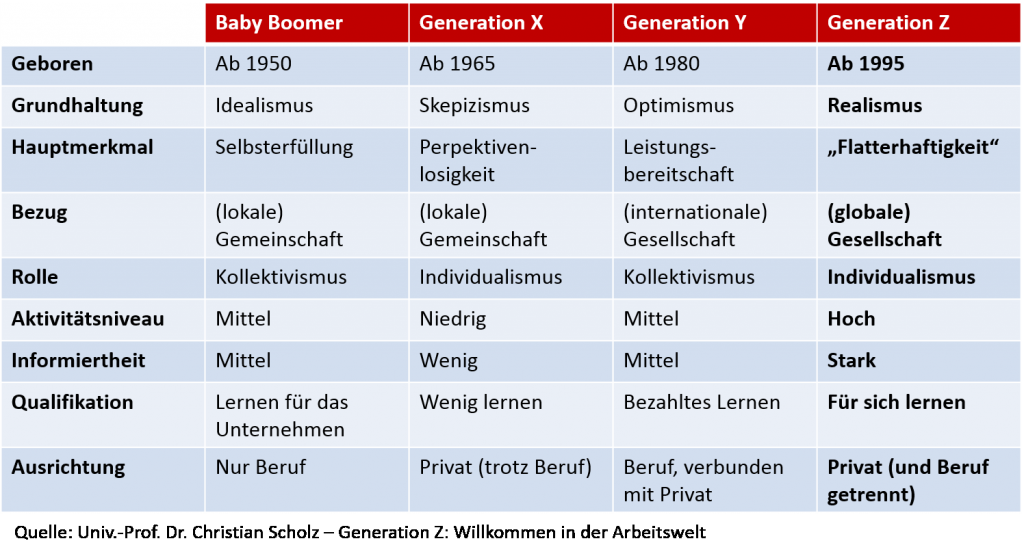
\includegraphics[width=1.0\textwidth]{Generationentabelle.png}\\
  Source: \cite{GenZ}
\end{center}
As shown in the graphic, Generation Z prefers a fixed salary. This matches
their individual aims. A high income is not that important. This is completely
different for Generation Y. A fixed salary can lead to lack of productivity
and motivation. An individual income is seen as appreciation of the own
achievements. To satisfy the different needs of different generations, new
compensation systems are evolving.

\subsection{Cafeteria Systems}
The idea of the cafeteria systems is to individualize payments. All employees
can choose whether they want more holidays or a higher income. It is also
possible to cut down the weekly working time and lower the income. These
systems are pretty popular in the US, where health insurance and other social
benefits are not obligatory by law. Employees can individualize their
compensation model to the maximum corresponding to their private and financial
situation. On the other hand are cafeteria systems linked with a high
administration effort \cite{HOLTB}.

\subsection{Current Trends in Compensation}
New generations insist on new working models and payment ideas. Therefore
companies are in need to create new ways to handle these new generations of
employees. This lead to the term "new pay". New Pay focuses on more
participation of the employees in creating new payment systems, is open for
new kinds and alternative ways of incentives, like days off, sabbaticals,
trainings and workshops instead of cash \cite{NewPay}.
\clearpage
\raggedright
\begin{thebibliography}{xxx}
\bibitem{WIRLEX} Gabler Wirtschaftslexikon; Zuletzt aufgerufen am 01.05.21
  \url{https://wirtschaftslexikon.gabler.de/definition/genfer-schema-32895/version-256426}

\bibitem{HOLTB} Dirk Holtbrügge, Jonas F. Puck. Personalmanagement.  Springer
  Berlin Heidelberg, 2005.

\bibitem{HAY} HayGroup. Hay Group guide chart and profile method of job
  evaluation -- an introduction and overview, 2012.
  \url{https://www.fahr.gov.ae/Portal/Userfiles/Assets/Documents/41ca116e.pdf}

\bibitem{HBS} Marion Weckes, Qendresa Berisha. Manager to Worker Pay Ratio --
  Mitbestimmungsreport. Hans Böckler Stiftung, 2016
  \url{https://www.boeckler.de/de/faust-detail.htm?sync_id=HBS-006451}

\bibitem{FORBES} Jesse Colombo. Why Has The U.S. CEO-To-Worker Pay Ratio
  Increased So Much? Forbes, 2019.
  \url{https://www.forbes.com/sites/jessecolombo/2019/08/31/why-has-the-u-s-ceo-to-worker-pay-ratio-increased-so-much/?sh=7b121f1b455e}

\bibitem{VI} Eidgenössische Volksinitiative '1:12 - Für gerechte Löhne, 2013.
  \url{https://www.bk.admin.ch/ch/d/pore/vi/vis375.html}

\bibitem{Solbach} Jonas Solbach. Zeit zum Umdenken.  HSG Focus 3/2019.
  \url{https://magazin.hsgfocus.ch/hsg-focus-3-2019-20gesundheit/artikel/boni-und-motivation-zeit-zum-umdenken-14412}

\bibitem{GenZ} Christian Scholz. Festlohnprinizip für Gen-Z. Generation-Z,
  2014.  \url{http://die-generation-z.de/festlohnprinzip-fuer-gen-z/}

\bibitem{NewPay} Sven Franke, Stefanie Hornung, Nadine Nobile. New Pay --
  Alternative Arbeits- und Entlohnungsmodelle. Haufe Lexware, 2019. ISBN
  978-3-648-11725-5.
\end{thebibliography}

\end{document}
